\begin{figure}[ht]
    \centering
    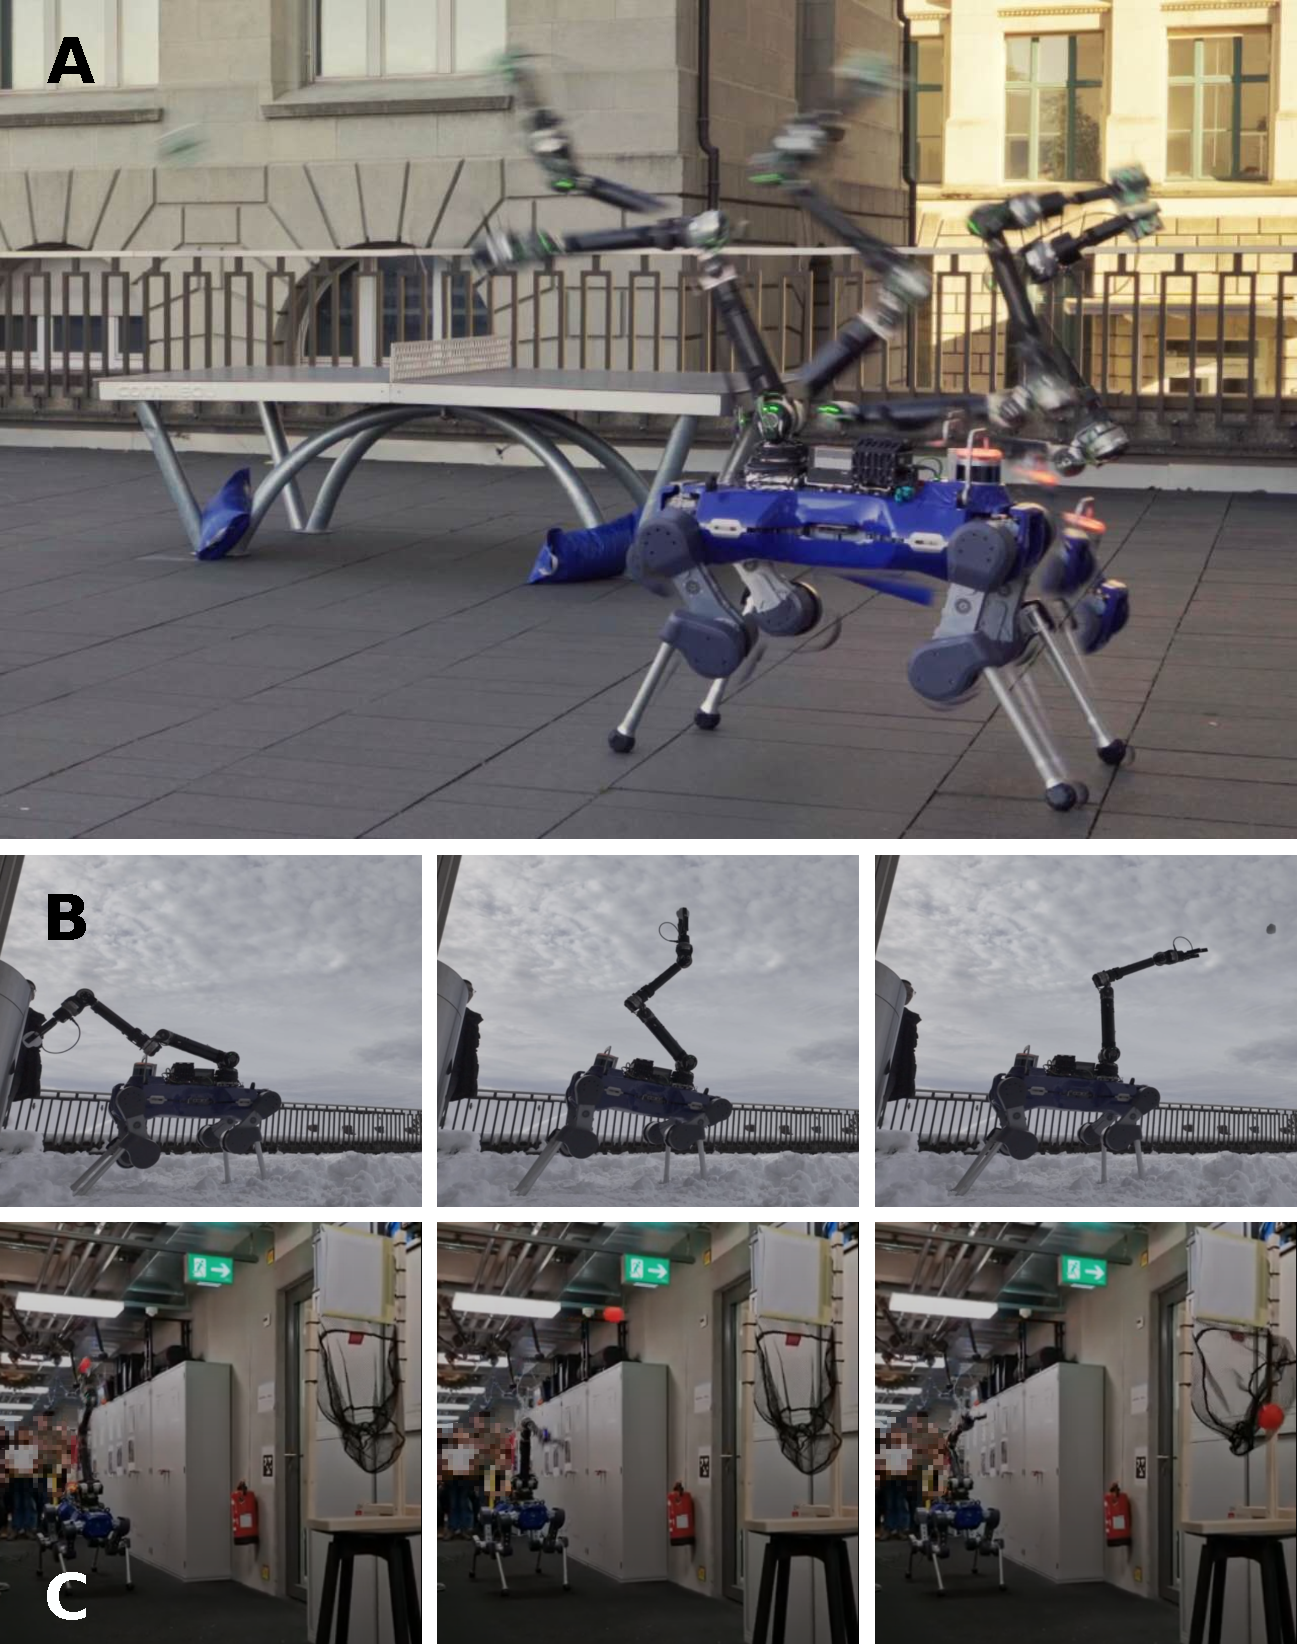
\includegraphics[width=0.48\textwidth]{figures/collage/collage1.pdf}
    \caption{\textbf{The robot performing prehensile whole-body throwing with varying velocities and object properties. (A)} A gift box. \textbf{(B)} A snowball. \textbf{(C)} A floorball. The target positions for the throws are identified using AprilTags, and the EE throwing states are calculated based on a user-specified velocity component along the $x$-axis, aligned with the robot's forward direction.}
    \label{fig:collage}
    
    % \vspace{1.5cm}
\end{figure}
